% =====================================================================================================
\section{Study 2: Effects of Individual Questions}\label{sec:study2}

\subsection{Design}
Study 1 measures the cumulative effect of four rounds of strategic play. Study 2 estimates the effect of a
\emph{single} question-selection decision by sampling continuations for every question in a generated candidate set. For each main case we take decision points at round $t=1$ (empty transcript) and $t=3$ (the
first two rounds of the Study-1 game in which both sides choose at random, separately for each type). The advocate
generator proposes $K=8$ candidate questions. For each candidate we
\begin{enumerate}
\item compute the lookahead planner's scores under \emph{two} internal judges, GPT-4o-mini and DeepSeek-V4-Flash,
using separately requested hypothetical guilty and innocent replies from the same simulator, with incomplete
sharing through the cache; and
\item realise the candidate $M=2$ times with independent continuations: the real defendant answers, and play continues
to round~4 with random selection on both sides. At $t=1$ the prosecutor cannot see the type, so the same eight
candidates are realised for both twins.
\end{enumerate}
The judges then score every continuation immediately after the branched exchange (\emph{immediate} outcome, primary)
and after round 4 (\emph{final} outcome, a test of persistence). For each decision point and defendant type, the two continuations give an estimate
$\widehat V_j^e$ of each candidate's mean score under evaluator $e$. We evaluate specified selection rules
using the estimates for their selected candidates, averaging over ties: random choice (the mean of $\widehat V_j^e$), introspection, either planner, best-of-$k$
for every $k\le8$ (averaged over all $\binom{8}{k}$ subsets), and a \emph{split-sample selection benchmark} that selects on one
continuation and is evaluated on the other.

For a fixed state and candidate set, let $S$ denote the information used by a prespecified selection rule,
$J(S)$ its selected candidate, and $\mu_j^e$ the expected evaluation score for candidate $j$. If the evaluation
continuations are independent of the selection information and have stable response laws, then
\begin{equation}
\E[\widehat V_j^e\mid S]=\mu_j^e
\quad\Longrightarrow\quad
\E[\widehat V_{J(S)}^e\mid S]=\mu_{J(S)}^e.
\end{equation}
This supports unbiased evaluation of the specified rule under those conditions; it does not justify choosing a
rule after inspecting the same evaluation outcomes. The planner can still select poorly because its own scores
are noisy or misspecified. Only the eight generated candidates are evaluated, with two continuations each, so
neither their expected values nor the values of arbitrary utterances are known exactly. Effects at $t=3$ concern
states reached by the baseline policies, not the distribution of states induced by deploying a new policy throughout.

The split-sample benchmark chooses using one realised continuation and evaluates on the other, then swaps their
roles and averages. It estimates the performance of that noisy selection procedure, not the maximum of the true
candidate means. It therefore supplies a comparison with outcome-informed selection, not an upper bound.

Crossing the planner's internal judge with the evaluator gives a $2\times2$ comparison of matched pairs
(GPT-4o-mini$\to$GPT-4o-mini, DeepSeek$\to$DeepSeek) and mismatched pairs. Scores are divided by each evaluator's
mean between-candidate standard deviation, estimated from the observed continuations. The interaction contrast
cancels additive planner and evaluator main effects on this scale, but does not eliminate every form of
scale dependence or identify a unique mechanism of judge exploitation. The reported intervals treat these
estimated scale factors as fixed. H7--H9 test the selection gain, crossover interaction and gain per doubling of
the candidate subset size (\cref{tab:confirm}).

\subsection{Results}
Of the 144 planned decision points, \StwoNfail{} failed after retries (malformed candidate output) and were excluded as
pre-specified, leaving \StwoNpoints{} decision points and \StwoNcont{} realised continuations.

\paragraph{A single strategic move.}
Choosing among the same eight candidates with the GPT-4o-mini planner raised the immediate probability of guilt under
GPT-4o-mini by \HSevenImmediate{} points over random choice (H7). The split-sample selection benchmark gained \SelOracleImmediate{}, providing a comparison with selection
using a separately realised outcome. Introspection over the same candidates gained \SelIntroImmediate{}.
Candidate values were moderately reliable across the two independent realisations ($r=\RelImmediateA$ for
GPT-4o-mini, \RelImmediateE{} for DeepSeek), indicating some reproducible variation between questions alongside continuation noise.

\paragraph{Planner--evaluator interaction.}
\Cref{fig:s2} (centre) shows the $2\times2$ crossover in standardised units. The GPT-4o-mini planner's picks were
worth \CrossAA\,SD to GPT-4o-mini but only \CrossAE\,SD to DeepSeek. The DeepSeek planner's picks were worth \CrossEA{}
and \CrossEE\,SD to GPT-4o-mini and DeepSeek respectively; its internal signal is a noisier stated probability, test--retest $r=\RetestER$. The specified
interaction (matched minus mismatched) was \HEightImmediate{}\,SD (H8, $p_{\text{Holm}}\HolmHEight$). The planners'
scores tell the same story: within a decision point, the GPT-4o-mini planner's scores correlated
$\rho={}$\ValImmAtoA{} with realised values under GPT-4o-mini but only \ValImmAtoE{} under DeepSeek. Introspection,
which models no particular judge, had a larger estimated gain than the cross-judge planner: \SelIntroImmediate{} under
GPT-4o-mini and \SelIntroImmediateE{} under DeepSeek, against \SelLookAAdvOnEImmediate{} for the GPT-4o-mini planner
evaluated by DeepSeek. This is the move-level counterpart of the transfer gap in Study 1 (H6), expressed as an
interaction on the chosen standardised scale.

\begin{figure}[t]
\centering
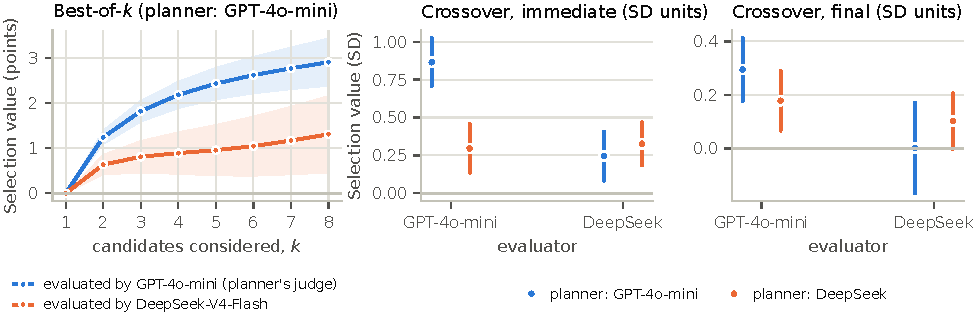
\includegraphics[width=\linewidth]{figs/s2_dose_crossover.pdf}
\caption{Study 2. \emph{Left:} value of choosing the best of $k$ candidates by the GPT-4o-mini planner, over random
choice, for the immediate outcome; expectations over all $\binom{8}{k}$ subsets with 95\% bands across cases. The
same choices are worth less than half as much to a different judge. \emph{Centre and right:} planner $\times$
evaluator crossover in each evaluator's between-candidate SD units, for the immediate and final outcomes; matched pairs
are the planner's own judge.}
\label{fig:s2}
\end{figure}

\paragraph{Dose-response.}
The value of selection rose concavely with the number of candidates considered (\cref{fig:s2}, left): by
\HNineImmediate{} points per doubling of $k$ (H9). Gains diminished from the second candidate onwards, and the curve
for the non-modelled judge was flatter throughout. Within these candidate sets, selecting from larger subsets improved the modelled judge's score more than
the other evaluator's score.

\paragraph{Persistence.}
Strategic moves fade. The immediate advantage of \HSevenImmediate{} shrank to \HSevenFinal{} points by round~4. For
first-round moves it fell from \PersistOneImm{} to \PersistOneFin{}, and for third-round moves from \PersistThreeImm{}
to \PersistThreeFin{}. By round~4 the realised value of a candidate was barely reproducible across its two
continuations ($r=\RelFinalA$), and the split-sample benchmark, which selects on a single noisy realisation, showed no clear gain over random choice
(\SelOracleFinal{}), whereas the planner, which selects on an independent signal, still did. Early moves had the larger immediate effect, consistent with the steep first-round drift in \cref{fig:drift}.
The decline shows that a local selection gain need not persist under the baseline continuation policy; it does not
decompose the cumulative policy effect in Study 1.

\paragraph{Selection for discrimination.}
At $t=1$ the same eight questions were realised for both twins, so each question's discriminating power, $D_j$
(guilty minus innocent), can be measured directly. The split-sample benchmark increased estimated immediate discrimination by \DiscSplitOracleA{} points under GPT-4o-mini. Choosing by the minister's
simulated score $\hat p_\G-\hat p_\I$ gained only \DiscMinPickA{}. This comparison suggests that the candidate sets contained useful variation that the minister's simulated
scores captured poorly. A possible explanation is mismatch between the hypothetical respondents, who improvise
from the public file, and defendants with case-specific private briefs. The experiment does not isolate this
explanation from other limitations of the planner.
